\documentclass[a4paper, 12pt]{report}
\usepackage{cmap}
\usepackage[T2A]{fontenc}
\usepackage[utf8]{inputenc}
\usepackage[english,russian]{babel}
\usepackage{listings}
\usepackage{amsmath}
\usepackage{float}
\usepackage{csquotes}
\usepackage{graphicx}
\graphicspath{ {./images/} }
\usepackage{xcolor}
\definecolor{buzzlightyear}{HTML}{8757A5}
\definecolor{grass}{HTML}{738D06}
\definecolor{literal}{HTML}{F18A2B}
\definecolor{commentcolor}{HTML}{8E908B}

\lstdefinestyle{habrstyle}{
	backgroundcolor=\color{white},
	commentstyle=\color{commentcolor},
	keywordstyle=\bfseries\color{buzzlightyear},
	numberstyle=\tiny\color{commentcolor},
	stringstyle=\color{grass},
	basicstyle=\ttfamily\footnotesize,
	breakatwhitespace=false,         
    	breaklines=true,                 
   	captionpos=b,                    
    	keepspaces=true,                 
    	numbers=left,                    
    	numbersep=7pt,                  
    	showspaces=false,                
    	showstringspaces=false,
   	showtabs=false,                  
    	tabsize=4
}

\lstset{style=habrstyle}

\author{3530901/80201, Шелаев Н. Р.}
\title{Лабораторная работа № 3. Апериодические сигналы.}
\date{\today}

\begin{document}
	\maketitle
	\tableofcontents
	\listoffigures
	\lstlistoflistings

	\chapter{Линейный чирп}
	Строим линейный чирп.
	\begin{lstlisting}[language=Python,caption=Линейный чирп]
		from thinkdsp import Chirp

		signal = Chirp(start = 220, end = 880)
		wave = signal.make_wave(duration = 2)
		wave.segment(start = 0, duration = 0.01).plot()
		wave.segment(start = 0.9, duration = 0.01).plot()
	\end{lstlisting}
	\begin{figure}[H]
		\centering
		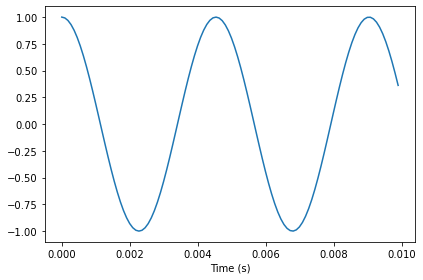
\includegraphics[width=0.75\textwidth]{chirp1.png}
		\caption{Начало сигнала}
		\label{fig:chirp1}
	\end{figure}
	\begin{figure}[H]
		\centering
		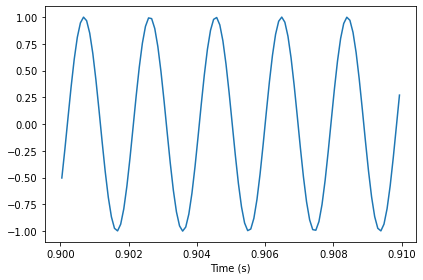
\includegraphics[width=0.75\textwidth]{chirp2.png}
		\caption{Конец сигнала}
		\label{fig:chirp2}
	\end{figure}
	\begin{lstlisting}[language=Python,caption=Строим спектр чирпа]
		signal = Chirp(start = 220, end = 440)
		wave = signal.make_wave(duration = 1)
		spectrum = wave.make_spectrum()
		spectrum.plot(high = 700)
	\end{lstlisting}
	\begin{figure}[H]
		\centering
		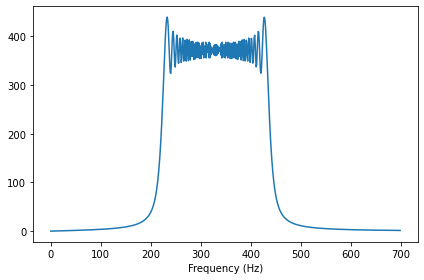
\includegraphics[width=0.75\textwidth]{chirp3.png}
		\caption{Спектр чирпа}
		\label{fig:chirp3}
	\end{figure}
	Слушая этот чирп, мы заметили, что высота звука сначала резко нарастает, а затем рост замедляется.

	\chapter{Спектрограмма}
	Знакомимся с одним из способов визуализации кратковременного преобразования Фурье (КВПФ).
	\begin{lstlisting}[language=Python,caption=Функция для построения спектрограммы]
		def plot_spectrogram(wave, seg_length):
			spectrogram = wave.make_spectrogram(seg_length)
			print('Time resolution (s)', spectrogram.time_res)
			print('Frequency resolution (Hz)', spectrogram.freq_res)
			spectrogram.plot(high = 700)
			decorate(xlabel = 'Time(s)', ylabel = 'Frequency (Hz)')
		
		signal = Chirp(start = 220, end = 440)
		wave = signal.make_wave(duration=1, framerate=11025)
		plot_spectrogram(wave, 512)
	\end{lstlisting}
	\begin{figure}[H]
		\centering
		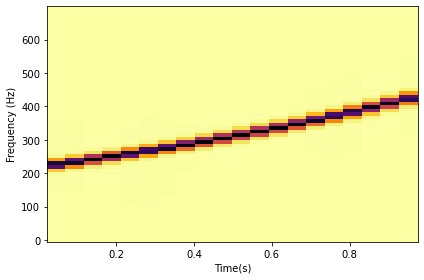
\includegraphics[width=0.75\textwidth]{chirp4.png}
		\caption{Спектрограмма чирпа}
		\label{fig:chirp4}
	\end{figure}
	Разрешение по времени спектрограммы зависит от длительности сегментов, соответствующих ширине ячеек спектрограммы.
	Разрешение по частоте спектрограммы - это частотный интервал между элементами спектра с одинаковой высотой ячеек.

	\chapter{Утечки}
	Знакомимся с утечками сигнала и способами их убрать.
	\begin{lstlisting}[language=Python,caption=Спектр сигнала]
		from thinkdsp import SinSignal

		signal = SinSignal(freq = 440)
		duration = signal.period * 30.25
		wave = signal.make_wave(duration)
		wave.plot()
		spectrum = wave.make_spectrum()
		spectrum.plot(high = 880)
	\end{lstlisting}
	\begin{figure}[H]
		\centering
		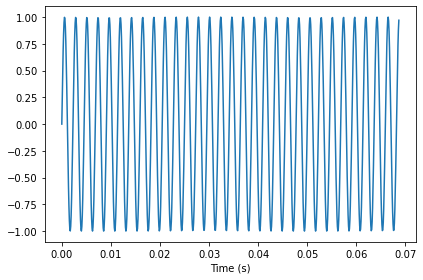
\includegraphics[width=0.75\textwidth]{leak1.png}
		\caption{Полученный сигнал}
		\label{fig:leak1}
	\end{figure}
	\begin{figure}[H]
		\centering
		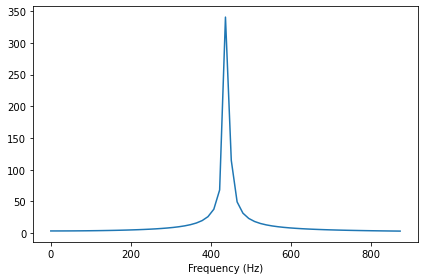
\includegraphics[width=0.75\textwidth]{leak2.png}
		\caption{Сегмент сигнала с утечкой}
		\label{fig:leak2}
	\end{figure}
	\begin{lstlisting}[language=Python,caption=Исправление сигнала функцией Хэмминга]
		wave.hamming()
		spectrum = wave.make_spectrum()
		spectrum.plot(high = 880)
	\end{lstlisting}
	\begin{figure}[H]
		\centering
		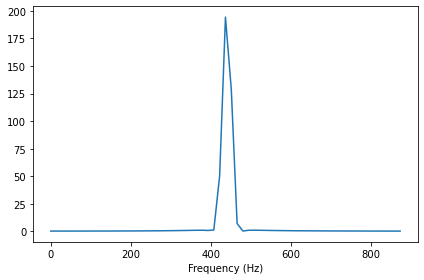
\includegraphics[width=0.75\textwidth]{leak3.png}
		\caption{Исправление утечки}
		\label{fig:leak3}
	\end{figure}

	\chapter{Упражнения}
	\section{Задание 1}
	Использование различных функций для исправления утечки сигнала.
	\begin{lstlisting}[language=Python,caption=Борьба с утечкой]
		for window_func in [np.bartlett, np.blackman, np.hamming, np.hanning]:
			wave = signal.make_wave(duration)
			wave.ys *= window_func(len(wave.ys))
			spectrum = wave.make_spectrum()
			spectrum.plot(high = 880, label = window_func.__name__)
	\end{lstlisting}
	\begin{figure}[H]
		\centering
		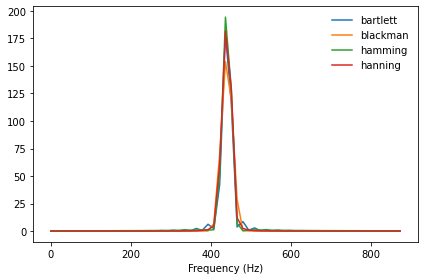
\includegraphics[width=0.75\textwidth]{leak4.png}
		\caption{Исправление утечки различными функциями}
		\label{fig:leak4}
	\end{figure}
	Все 4 функции хорошо справляются с уменьшением утечки, но фильтр Хэмминга рассеивает наименьшее количество энергии.

	\section{Задание 2}
	Пилообразный сигнал с линейно увеличивающейся (или уменьшающейся) частотой.
	\begin{lstlisting}[language=Python,caption=Создание нового класса]
		from thinkdsp import normalize, unbias

		class SawtoothChirp(Chirp):

			def evaluate(self, ts):
				freqs = np.linspace(self.start, self.end, len(ts))
				dts = np.diff(ts, prepend = 0)
				dphis = self.PI2 * freqs * dts
				phases = np.cumsum(dphis)
				cycles = phases / self.PI2
				frac, _ = np.modf(cycles)
				ys=normalize(unbias(frac), self.amp)
				return ys
		
		signal = SawtoothChirp(start = 220, end = 880)
		wave = signal.make_wave(duration=1, framerate=8000)
		wave.apodize()
		sp = wave.make_spectrogram(256).plot()
	\end{lstlisting}
	\begin{figure}[H]
		\centering
		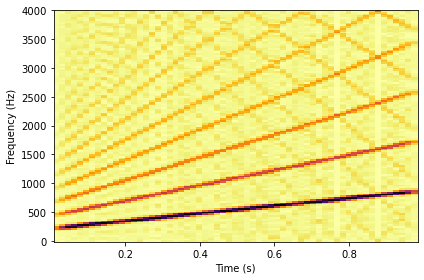
\includegraphics[width=0.75\textwidth]{chirp5.png}
		\caption{Спектрограмма полученного сигнала}
		\label{fig:chirp5}
	\end{figure}
	
	\section{Задание 3}
	Создание пилообразного чирпа.
	\begin{lstlisting}[language=Python,caption=Пилообразный чирп]
		signal = SawtoothChirp(start = 2500, end = 3000)
		wave = signal.make_wave(duration=1, framerate=20000)
		wave.make_spectrum().plot()
	\end{lstlisting}
	\begin{figure}[H]
		\centering
		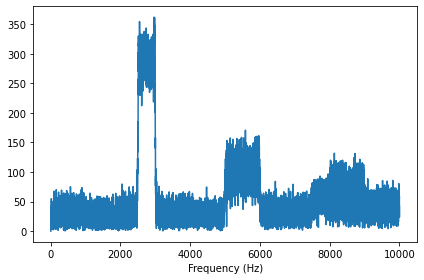
\includegraphics[width=0.75\textwidth]{chirp6.png}
		\caption{Спектр пилообразного чирпа}
		\label{fig:chirp6}
	\end{figure}	

	\section{Задание 4}
	Изучение сигнала \texttt{глиссандо}
	\begin{lstlisting}[language=Python,caption=Получение сигнала]
		wave=read_wave('72475__rockwehrmann__glissup02.wav')
		wave.make_audio()
		wave.make_spectrogram(512).plot(high = 5000)
	\end{lstlisting}
	\begin{figure}[H]
		\centering
		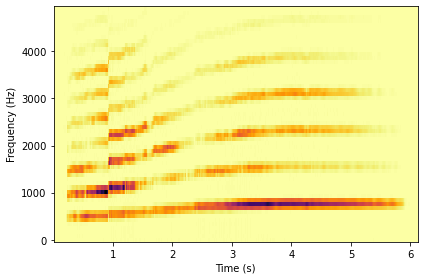
\includegraphics[width=0.75\textwidth]{glis1.png}
		\caption{Спектрограмма сигнала глиссандо}
		\label{fig:glis1}
	\end{figure}
	
	\section{Задание 5}
	Изменение частоты сигнала \texttt{глиссандо} во времени.
	\begin{lstlisting}[language=Python,caption=Новый класс для изменения частоты сигнала]
		class TromboneGliss(Chirp):
    
			def evaluate(self, ts):
				l1, l2 = 1.0 / self.start, 1.0 / self.end
				lengths = np.linspace(l1, l2, len(ts))
				freqs = 1 / lengths
				dts = np.diff(ts, prepend = 0)
				dphis = 2 * np.pi * freqs * dts
				phases = np.cumsum(dphis)
				ys = self.amp * np.cos(phases)
				return ys
	\end{lstlisting}
	\begin{lstlisting}[language=Python,caption=Получение требуемого сигнала]
		low = 262
		high = 349
		signal = TromboneGliss(high, low)
		wave1 = signal.make_wave(duration = 1)
		wave1.apodize()
		signal = TromboneGliss(low, high)
		wave2 = signal.make_wave(duration = 1)
		wave2.apodize()
		wave = wave1 | wave2
		sp = wave.make_spectrogram(1024)
		sp.plot(high = 1000)
	\end{lstlisting}
	\begin{figure}[H]
		\centering
		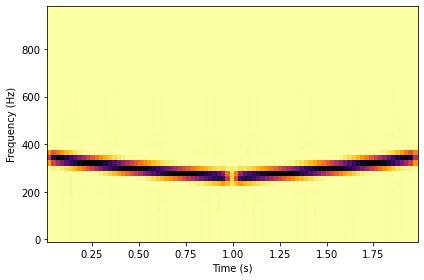
\includegraphics[width=0.75\textwidth]{test1.png}
		\caption{Спектрограмма полученного сигнала}
		\label{fig:test1}
	\end{figure}
	Полученная спектрограмма больше напоминает линейный чирп.	

	\section{Задание 6}
	Спектрограмма гласных звуков.
	 \begin{lstlisting}[language=Python,caption=Получение сигнала]
		wave = read_wave('87778__marcgascon7__vocals.wav')
		wave.make_spectrogram(1024).plot(high = 1000)
	\end{lstlisting}
	\begin{figure}[H]
		\centering
		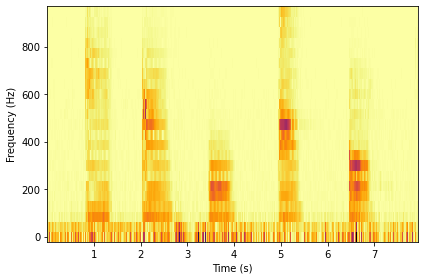
\includegraphics[width=0.75\textwidth]{test2.png}
		\caption{Спектрограмма 5 гласных звуков}
		\label{fig:test2}
	\end{figure}
	\begin{lstlisting}[language=Python,caption=Сегменты для каждого звука]
		segment = wave.segment(start = 1, duration = 0.25)
		wave.make_spectrogram(1024).plot(high = 1000)
		segment = wave.segment(start = 2.2, duration = 0.25)
		segment.make_spectrum().plot(high = 1000)
		segment = wave.segment(start = 3.5, duration = 0.25)
		segment.make_spectrum().plot(high = 1000)
		segment = wave.segment(start = 5.1, duration = 0.25)
		segment.make_spectrum().plot(high = 1000)
		segment = wave.segment(start = 6.5, duration = 0.25)
		segment.make_spectrum().plot(high = 1000)
	\end{lstlisting}
	\begin{figure}[H]
		\centering
		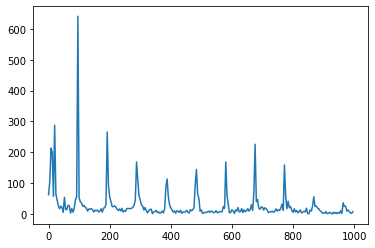
\includegraphics[width=0.75\textwidth]{word1.png}
		\caption{Сегмент со звуком A}
		\label{fig:word1}
	\end{figure}
	\begin{figure}[H]
		\centering
		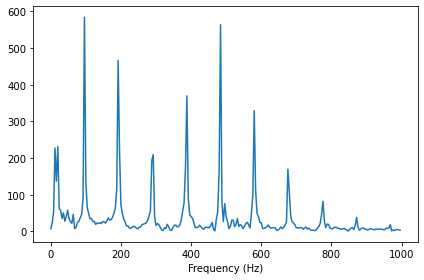
\includegraphics[width=0.75\textwidth]{word2.png}
		\caption{Сегмент со звуком Э}
		\label{fig:word2}
	\end{figure}
	\begin{figure}[H]
		\centering
		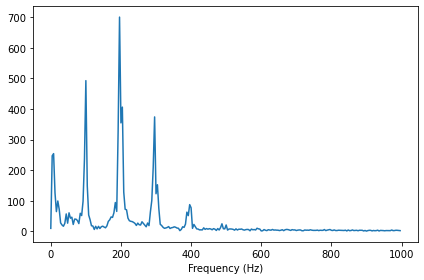
\includegraphics[width=0.75\textwidth]{word3.png}
		\caption{Сегмент со звуком И}
		\label{fig:word3}
	\end{figure}
	\begin{figure}[H]
		\centering
		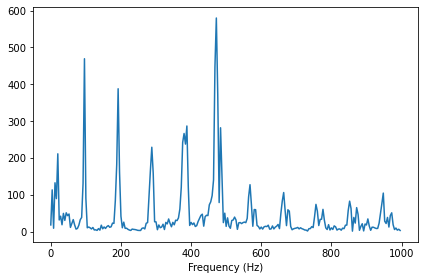
\includegraphics[width=0.75\textwidth]{word4.png}
		\caption{Сегмент со звуком О}
		\label{fig:word4}
	\end{figure}
	\begin{figure}[H]
		\centering
		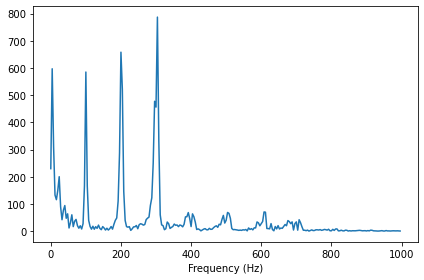
\includegraphics[width=0.75\textwidth]{word5.png}
		\caption{Сегмент со звуком У}
		\label{fig:word5}
	\end{figure}
	По спектрограммам и сегментам очень сложно определить гласную.

	\chapter{Вывод}
	В данной работе мы познакомились с сигналом \texttt{чирпа}, спектрограммами и утечками сигналов. Утечки сигналов можно уменьшить, если использовать различные виды \texttt{окон}. В конце увидели спектрограмму 5 разных гласных звуков.
\end{document}